%% The first command in your LaTeX source must be the \documentclass command.
\documentclass[]{ceurart}
\sloppy
\usepackage{listings}
\lstset{breaklines=true}
\usepackage{graphicx}
\usepackage{booktabs}

\begin{document}
\copyrightyear{2025}
\copyrightclause{Copyright for this paper by its authors.
  Use permitted under Creative Commons License Attribution 4.0
  International (CC BY 4.0).}
\conference{AdvAIT'2025: 2nd International Workshop on Advanced Applied Information Technologies, December 5, 2025, Khmelnytskyi, Ukraine}

\title{Method of knowledge integration for segmentation of heart regions based on its MRI image: a standards-compliant, ONNX-portable, and graph-based approach validated on ACDC and M\&Ms-2}

\author[1]{Oleksandr Chaban}[orcid=0009-0001-4710-3336,email={chabanolek@khmnu.edu.ua},]
\author[1]{Eduard Manziuk}[orcid=0000-0002-7310-2126,email={manziuk.e@khmnu.edu.ua},]
\author[1]{Pavlo Radiuk}[orcid=0000-0003-3609-112X,email={radiukp@khmnu.edu.ua},]
\cormark[1]
\author[2]{Olena Markevych}[orcid=0000-0003-2758-3288,email={elena--14@ukr.net},]

\address[1]{Khmelnytskyi National University, 11, Institutes str., Khmelnytskyi, 29016, Ukraine}
\address[2]{Khmelnytskyi Infectious Diseases Hospital, 17, Skovorody str., Khmelnytskyi, 29008, Ukraine}

\cortext[1]{Corresponding author.}

\begin{abstract}
Cardiac magnetic resonance imaging (MRI) enables precise quantification of ventricular structure and function, but operationalizing research prototypes as dependable clinical tools remains difficult. Deployments must ingest heterogeneous DICOM/NIfTI data while preserving geometry and privacy, run models efficiently on CPUs and GPUs from different vendors, and generate decisions that clinicians can interpret and audit. In this work, we propose a method of knowledge integration for segmentation of heart regions based on its MRI image that unifies standards‑compliant DICOM/NIfTI ingestion with de‑identification, portable ONNX Runtime inference, and a graph‑based classifier that reasons over mask‑derived cardiac measurements. On ACDC and M&Ms‑2 we obtain competitive segmentation (macro Dice 0.939 and 0.927, respectively) and robust diagnosis (94.0% accuracy; macro ROC‑AUC ≈0.964; macro PR‑AUC ≈0.951). Relative to a strong U‑Net baseline, our segmentation improves myocardium Dice by +1.7 points and reduces HD95 by ≈1.7 mm. Temperature scaling lowers Brier (0.08→0.07) and ECE (0.04→0.03), supporting trustworthy deployment. The significant conclusion is that combining explicit domain knowledge with standards‑aware engineering yields a portable, auditable, and calibrated system that closes the gap between algorithmic performance and clinical reliability.
\end{abstract}

\begin{keywords}
Cardiac MRI, Segmentation, Knowledge Integration, Graph Neural Networks, ONNX Runtime, DICOM, Calibration
\end{keywords}

\maketitle


\section{Introduction}
Cardiac magnetic resonance imaging (MRI) is the modality of choice for quantifying ventricular morphology and function. 
Accurate delineation of the left‑ventricular (LV) cavity, right‑ventricular (RV) cavity, and myocardium (Myo) underpins the computation of clinically salient indices—end‑diastolic and end‑systolic volumes, ejection fraction, stroke volume, and wall thickness—that guide diagnosis and treatment. 
Despite the maturity of modern segmentation architectures, transferring research models into real clinical software remains challenging because the full pipeline must satisfy three constraints simultaneously: (i) \emph{interoperability and privacy}, (ii) \emph{hardware portability and predictable latency}, and (iii) \emph{interpretability and calibration}. 
Clinical data arrive as Digital Imaging and Communications in Medicine (DICOM) series with protected health information (PHI) that must be removed or pseudonymized, or as research‑oriented Neuroimaging Informatics Technology Initiative (NIfTI) volumes whose affine geometry and orientation must be honored to avoid subtle mis‑registration. 
Deployment requires models to execute efficiently across CPUs and different GPU vendors without vendor lock‑in, a requirement naturally addressed by the Open Neural Network Exchange (ONNX) format and ONNX Runtime execution providers (EPs). 
Finally, downstream diagnostic decisions must be expressed in a manner that clinicians can audit, and the system must record its actions for reproducibility and regulatory review.

This paper advances a principled solution rooted in \emph{knowledge integration}. 
We inject domain knowledge at multiple levels of the pipeline: we enforce standards during data handling and log all privacy actions; we design a segmentation module (SKIF‑Seg) that encodes anatomy‑aware priors through its preprocessing and post‑processing; and we perform diagnosis using a graph neural network (KI‑GCN) that operates on interpretable, mask‑derived measurements and encodes clinical relations as edges. 
The result is a portable, standards‑aware, and calibrated system that demonstrates strong accuracy on two public benchmarks and documents every run for reproducible science.

\subsection{Motivation and contributions}
A recurring obstacle in clinical adoption of AI is the disconnect between high scores on public leaderboards and the operational realities of hospital software. 
First, \textbf{data interoperability and privacy}. 
DICOM governs the semantics and transport of medical images and mandates careful handling of identifiers; correct de‑identification must remove or replace PHI while retaining acquisition parameters and measurement‑critical metadata. 
NIfTI, the de‑facto research standard for 3D/4D volumes, embeds voxel spacing and orientation in an affine header; errors here silently invalidate geometric comparisons~\cite{dicom_ps3_1,nifti_site}. 
Second, \textbf{hardware portability}. 
Research code often targets a single framework and GPU vendor; clinical systems operate across CPUs and diverse GPUs (or no GPU at all). 
Exporting networks to ONNX and executing them with ONNX Runtime EPs (CPU, CUDA, DirectML) alleviates these constraints and ensures predictable latency across sites~\cite{onnxruntime_docs,cuda_guide,directml_docs}. 
Third, \textbf{interpretability and calibration}. 
Diagnosis must be explainable in terms of familiar quantities, and predicted probabilities must be reliable; uncalibrated over‑confidence undermines trust~\cite{niculescu2005calibration,brier1950}.

\textbf{This paper makes three contributions.} 
(1) We design a \emph{standards‑aware, manifest‑driven} pipeline: DICOM/NIfTI ingestion with de‑identification, geometry‑preserving preprocessing, and automatic manifest logging of software versions, ONNX opsets, EP choice, hashes, and metrics. 
(2) We introduce \emph{KI‑GCN}, a knowledge‑integrated graph classifier built on node features derived from segmentation masks; edges encode spatial adjacency and clinical heuristics, enabling context‑aware diagnosis~\cite{kipf2017gcn}. 
(3) We propose a \emph{deployment‑oriented evaluation} that combines classical segmentation metrics (Dice, HD95, ASSD) with discrimination (ROC‑AUC, PR‑AUC) and calibration (Brier, ECE with reliability diagrams), reflecting real operational needs~\cite{taha2015metrics,saito2015prauc}.

\subsection{State of the art}
U‑Net established the encoder–decoder template with skip connections that preserve spatial detail~\cite{ronneberger2015unet}. 
nnU‑Net raised this baseline through automated dataset‑specific configuration of data handling, architecture, training, and post‑processing, achieving reliable performance across diverse tasks~\cite{isensee2021nnunet}. 
Recent work explores Transformer‑inspired scaling of ConvNets (MedNeXt) and fully Transformer‑based volumetric segmentation (UNETR/UNETR++), trading off accuracy, efficiency, and memory~\cite{roy2023mednext}. 
For reasoning beyond pixel‑wise segmentation, graph neural networks (GNNs) propagate messages over a graph of entities; graph convolutional networks (GCNs) use normalized adjacency to perform neighborhood averaging, while graph attention networks (GATs) learn attention weights over neighbors~\cite{kipf2017gcn,velivckovic2018gat}. 
Calibration research stresses that reliable probabilities are as critical as discrimination, and simple temperature scaling is often sufficient to correct over‑confidence~\cite{niculescu2005calibration}.

\subsection{Previous works}
Our technical report presented an early prototype integrating DICOM/NIfTI handling, an ONNX‑exported segmentation model, and a diagnosis module consuming mask‑derived features. 
It emphasized the need for anonymization, execution‑provider benchmarking, and run manifests for auditability. 
The present paper formalizes the mathematical underpinnings of the segmentation and graph‑based diagnosis modules, revises the training and evaluation protocol, and adds cross‑center generalization experiments on M\&Ms‑2 together with a detailed calibration study.

\subsection{Purposes and objectives of the study}
\textbf{The goal of this study is to improve knowledge integration fidelity and downstream diagnostic reasoning by unifying standards‑compliant ingestion, portable ONNX inference, and graph‑structured classification with calibration‑aware evaluation.} 
To achieve this goal we: (i) implement a standards‑aware ingestion/anonymization module and a manifest‑driven export subsystem; (ii) design SKIF‑Seg and KI‑GCN to encode anatomical priors in both segmentation and diagnosis; and (iii) validate accuracy, generalization, and calibration on ACDC and M\&Ms‑2.



\section{Related Works}
\subsection*{Segmentation architectures}
Encoder–decoder networks remain the dominant approach for cardiac MRI segmentation. 
U‑Net’s symmetric architecture and skip connections improved delineation with limited annotation budgets~\cite{ronneberger2015unet}. 
nnU‑Net subsequently transformed lessons from dozens of challenges into rules for spacing selection, patch sizes, network depth, losses, and post‑processing, delivering strong “out‑of‑the‑box” baselines across modalities and anatomies~\cite{isensee2021nnunet}. 
In parallel, MedNeXt introduced large‑kernel ConvNeXt blocks customized for 3D medical images, offering a compelling accuracy–efficiency trade‑off and competitive performance to hybrid Transformer designs~\cite{roy2023mednext}.

\subsection*{Knowledge‑aware reasoning}
While many clinical pipelines stop at segmentation, diagnosis often benefits from explicit reasoning over structured quantities, such as volumes and ejection fractions. 
Graph neural networks provide a natural abstraction: nodes represent anatomical structures or cardiac phases, and edges encode spatial adjacency or physiological couplings. 
GCNs perform localized spectral filtering via normalized adjacency, and GATs learn attention coefficients to modulate neighbor influence~\cite{kipf2017gcn,velivckovic2018gat}. 
Such models can elegantly incorporate domain knowledge by shaping adjacency weights or adding constraint losses, yielding interpretable decisions grounded in anatomy.

\subsection*{Calibration and evaluation}
Segmentation quality is commonly measured with overlap (Dice, IoU) and boundary metrics (HD95, ASSD)~\cite{taha2015metrics}. 
For classification, discrimination metrics (ROC‑AUC, PR‑AUC) must be complemented with calibration measures because over‑confident predictions impair clinical trust. 
Brier score quantifies the mean squared error of probability forecasts~\cite{brier1950}, and reliability diagrams visualize the match between confidence and empirical accuracy. 
Temperature scaling on a held‑out split provides a simple post‑hoc fix that often improves calibration without altering discrimination~\cite{niculescu2005calibration}. 
PR‑AUC, in particular, is more informative than ROC‑AUC under label imbalance typical of multi‑class cardiac diagnoses~\cite{saito2015prauc}.

\subsection*{Objective and tasks}
The objective of this study is to \emph{operationalize knowledge integration} in a single system that respects standards, delivers strong segmentation, performs interpretable diagnosis, and reports calibrated probabilities. 
Our tasks are: (1) implement DICOM/NIfTI ingestion and anonymization with manifest logging; (2) execute segmentation via ONNX Runtime EPs (CPU, CUDA, DirectML) for cross‑hardware portability~\cite{onnxruntime_docs,cuda_guide,directml_docs}; (3) compute mask‑derived features and construct an anatomy‑aware cardiac graph; (4) train KI‑GCN with optional distillation and assess discrimination and calibration; and (5) validate robustness on ACDC and M\&Ms‑2~\cite{bernard2018acdc,campello2021mnms,martinisla2023mnms2}.



\section{Methods}
Figure~\ref{fig:pipeline} provides an overview of the pipeline. 
Raw series are ingested as DICOM or NIfTI, anonymized, and reoriented to a canonical layout; SKIF‑Seg performs volumetric segmentation using ONNX Runtime; interpretable features are computed from the masks and used to construct a domain‑informed cardiac graph; KI‑GCN performs diagnosis; and a manifest captures all relevant metadata for reproducibility.

\begin{figure}[!ht]
\centering
\includegraphics[width=0.98\linewidth]{figs/pipeline.png}
\caption{End‑to‑end workflow: standards‑compliant ingestion and anonymization; ONNX‑accelerated volumetric segmentation (SKIF‑Seg); feature extraction and graph construction; graph‑based diagnosis (KI‑GCN); and manifest‑driven export.}
\label{fig:pipeline}
\end{figure}

\subsection{Standards‑compliant ingestion and anonymization}
\textbf{DICOM.} Studies are read from disk as DICOM series. 
We reconstruct volumes from slices after validating series consistency (orientation, spacing, echo time) and apply a de‑identification profile that removes or replaces PHI, including \texttt{(0010,0010)} \emph{PatientName}, \texttt{(0010,0020)} \emph{PatientID}, and institutional identifiers. 
Non‑PHI acquisition parameters are retained to preserve scientific utility. 
All actions (removed tags, hashed tags, retained tags) are recorded in a JSON manifest with timestamps and software versions~\cite{dicom_ps3_1}. 
\textbf{NIfTI.} For research volumes, we parse the affine to obtain spacing, orientation, and origin, reorient volumes to a canonical RAS convention, and resample only as required to match the network’s target spacing. 
Intensities are normalized slice‑wise or volume‑wise using z‑score or min–max scaling depending on the training configuration~\cite{nifti_site}.

\subsection{Volumetric segmentation (SKIF‑Seg)}
SKIF‑Seg follows a 3D encoder–decoder topology with residual blocks and deep supervision. 
The model is exported to ONNX for inference and executed with ONNX Runtime. 
We expose three EPs: CPU for maximal compatibility, CUDA for NVIDIA GPUs, and DirectML for vendor‑neutral GPU acceleration on Windows~\cite{onnxruntime_docs,cuda_guide,directml_docs}. 
Let $V\!\in\!\mathbb{R}^{H\times W\times D}$ be the preprocessed volume. 
The network outputs a per‑voxel probability tensor $P\!\in\![0,1]^{H\times W\times D\times C}$ for $C{=}3$ classes (LV, Myo, RV). 
The discrete mask $\hat{M}$ is obtained by $\hat{M}(i)=\arg\max_c P_c(i)$ with connected‑component cleanup and small‑island removal.

\subsection{Feature extraction and knowledge graph}
From $\hat{M}$ and phase labels we compute: LV/RV end‑diastolic (ED) and end‑systolic (ES) volumes, stroke volumes, ejection fractions, myocardium volume, surface area, and centers of mass. 
We construct a graph $G=(V,E)$ whose nodes $v\!\in\!V$ correspond to LV\_ED, LV\_ES, RV\_ED, RV\_ES, and Myo; edges encode spatial adjacency and physiologic coupling (e.g., LV\_ED↔LV\_ES, RV\_ED↔RV\_ES, LV↔Myo, RV↔Myo). 
Each node is associated with a feature vector $\mathbf{x}_v$ concatenating normalized measurements and optional demographic covariates when available. 
Edges may be re‑weighted by simple clinical heuristics; for instance, edges affecting LV volume dynamics receive higher weight for discriminating dilated cardiomyopathy.

\subsection{Graph‑based classifier (KI‑GCN)}
Let $X\!\in\!\mathbb{R}^{|V|\times d}$ be the stacked node features and let $\tilde{A}\!=\!A+I$ add self‑loops. 
We apply $L$ graph convolutional layers with
\begin{equation}
H^{(\ell+1)}=\sigma\!\left(\tilde{D}^{-1/2}\tilde{A}\,\tilde{D}^{-1/2}\,H^{(\ell)}W^{(\ell)}\right),\qquad H^{(0)}=X,
\end{equation}
where $\tilde{D}$ is the degree matrix of $\tilde{A}$ and $\sigma$ is ReLU~\cite{kipf2017gcn}. 
Global mean pooling yields $\mathbf{h}_G\!=\!\mathrm{mean}(H^{(L)})$, which is passed through a linear layer to predict logits $z\!\in\!\mathbb{R}^K$ for $K$ diagnostic classes (NOR, HCM, DCM, MINF, ARV). 
We optionally incorporate \emph{knowledge‑weighted graphs} by replacing $\tilde{A}$ with $\tilde{A}'$ whose entries reflect domain rules (e.g., higher LV\_ED↔LV\_ES weight).

\subsection{Distillation and calibration}
To deploy lightweight models, we train a student KI‑GCN with a blended objective against an ensemble of teachers:
\begin{equation}
\mathcal{L}=\alpha\,\mathcal{L}_{\mathrm{CE}}\!\left(y,\operatorname{softmax}\big(z^{(s)}\big)\right)
+(1-\alpha)\,\tau^2\,\mathrm{KL}\!\left(\operatorname{softmax}\!\frac{\bar{z}^{(t)}}{\tau}\;\Big\|\;\operatorname{softmax}\!\frac{z^{(s)}}{\tau}\right).
\end{equation}
Post‑hoc temperature scaling on a validation split calibrates probabilities prior to deployment. 
We report discrimination (accuracy, macro‑F1, ROC‑AUC, PR‑AUC) and calibration (Brier score, ECE with reliability diagrams)~\cite{niculescu2005calibration,brier1950,saito2015prauc}.

\subsection{Evaluation metrics and manifests}
For segmentation we compute Dice and Jaccard (IoU)
\begin{equation}
\mathrm{Dice}(X,Y)=\frac{2|X\cap Y|}{|X|+|Y|},\qquad
\mathrm{IoU}(X,Y)=\frac{|X\cap Y|}{|X\cup Y|},
\end{equation}
together with boundary metrics HD95 and ASSD~\cite{taha2015metrics}. 
Every run writes a manifest with software versions, git commit, ONNX opset, EP choice, and metrics, enabling strict auditability and cross‑site reproducibility.




\subsection{Implementation details and reproducibility}
Training uses Adam with a cosine schedule and mixed precision. 
Volumes are cropped to foreground using a bounding box with 10\% margin and patch‑wise training is adopted for memory efficiency. 
Augmentations include random intensity scaling and bias‑field simulation, small rotations ($\pm 10^\circ$), elastic deformations, and gamma adjustments. 
We use deep supervision and a compound Dice+Cross‑Entropy loss for segmentation; post‑processing applies connected‑component analysis and hole filling. 
For diagnosis, features are z‑normalized per cohort and missing values are imputed with cohort medians. 
We perform five‑fold cross‑validation to tune KI‑GCN depth ($L\in\{2,3,4\}$) and hidden width ($d\in\{32,64,128\}$). 
Each experiment writes a JSON manifest with software versions, ONNX opset numbers, EP selection, random seeds, dataset hashes, and all derived metrics and plots. 
Scripts provided with this paper reproduce every figure from CSV summaries and can be re‑run to regenerate artwork exactly.


\section{Results}
\subsection{Datasets and protocol}
The ACDC dataset provides short‑axis cine MRI with manual annotations for LV, Myo, and RV across five diagnostic categories (NOR, HCM, DCM, MINF, ARV)~\cite{bernard2018acdc}. 
The M\&Ms‑2 challenge extends multi‑center evaluation, focusing on RV segmentation with multi‑view acquisitions and diverse right‑heart pathologies~\cite{campello2021mnms,martinisla2023mnms2}. 
We train SKIF‑Seg on ACDC with a 70/10/20 split and evaluate in‑domain. 
For M\&Ms‑2, we apply the trained model with only intensity normalization and spacing adjustment; no target‑domain fine‑tuning is performed to stress generalization.

\subsection{Segmentation accuracy and robustness}
Table~\ref{tab:seg} reports per‑structure Dice/HD95 and complementary IoU/ASSD for SKIF‑Seg; a strong 3D U‑Net serves as the baseline. 
On ACDC, SKIF‑Seg improves myocardium Dice from 0.895 to 0.912 and reduces HD95 by nearly 2\,mm. 
Improvements are consistent for LV and RV. 
On M\&Ms‑2, accuracy remains high with small, uniform Dice drops (all within $[-0.013,-0.012]$), indicative of robust cross‑center transfer. 
Figure~\ref{fig:boxplots} shows case‑wise Dice distributions with narrower dispersion for myocardium, and Figure~\ref{fig:macro} summarizes macro Dice by dataset.

\begin{table}[!ht]
\centering
\caption{Per‑structure segmentation on ACDC (in‑domain) and M\&Ms‑2 (cross‑domain).}
\label{tab:seg}
\begin{tabular}{lcccccc}
\toprule
Dataset \& Structure & U\mbox{-}Net Dice & U\mbox{-}Net HD95 & SKIF\mbox{-}Seg Dice & SKIF\mbox{-}Seg IoU & SKIF\mbox{-}Seg HD95 & SKIF\mbox{-}Seg ASSD \\
\midrule
ACDC\,LV & 0.951 & 7.5 & 0.965 & 0.932 & 5.8 & 1.28 \\
ACDC\,Myo & 0.895 & 8.1 & 0.912 & 0.838 & 6.3 & 1.39 \\
ACDC\,RV & 0.930 & 9.2 & 0.941 & 0.889 & 7.7 & 1.69 \\
\midrule
M\&Ms\mbox{-}2\,LV & 0.942 & 8.9 & 0.953 & 0.911 & 7.2 & 1.58 \\
M\&Ms\mbox{-}2\,Myo & 0.881 & 9.8 & 0.899 & 0.817 & 7.9 & 1.74 \\
M\&Ms\mbox{-}2\,RV & 0.915 & 10.5 & 0.928 & 0.866 & 8.9 & 1.96 \\
\bottomrule
\end{tabular}
\end{table}

\begin{figure}[!ht]
\centering
\includegraphics[width=0.9\linewidth]{figs/seg_boxplots.png}
\caption{Case‑wise Dice distributions (SKIF‑Seg) across datasets and structures.}
\label{fig:boxplots}
\end{figure}

\begin{figure}[!ht]
\centering
\includegraphics[width=0.72\linewidth]{figs/seg_macro_bars.png}
\caption{Macro Dice across LV/Myo/RV for ACDC and M\&Ms‑2.}
\label{fig:macro}
\end{figure}

\subsection{Comparison with state of the art}
Table~\ref{tab:sota} compares SKIF‑Seg with nnU‑Net and MedNeXt. 
SKIF‑Seg is competitive with both methods—especially on myocardium (0.912)—while being embedded in a standards‑aware pipeline featuring anonymization, manifests, and cross‑hardware execution. 
This systems focus complements pure‑algorithmic advances~\cite{isensee2021nnunet,roy2023mednext}.

\begin{table}[!ht]
\centering
\caption{ACDC mean Dice comparison.}
\label{tab:sota}
\begin{tabular}{lcccc}
\toprule
Method & LV & Myo & RV & Mean Dice \\
\midrule
U\mbox{-}Net & 0.951 & 0.895 & 0.930 & 0.925 \\
nnU\mbox{-}Net~\cite{isensee2021nnunet} & \textbf{0.968} & 0.909 & \textbf{0.945} & \textbf{0.941} \\
MedNeXt~\cite{roy2023mednext} & 0.966 & 0.910 & 0.942 & 0.939 \\
\textbf{Proposed (SKIF\mbox{-}Seg)} & 0.965 & \textbf{0.912} & 0.941 & 0.939 \\
\bottomrule
\end{tabular}
\end{table}

\subsection{Generalization under domain shift}
Figure~\ref{fig:domain} quantifies Dice change (M\&Ms‑2 minus ACDC) per structure. 
All drops are small ($-0.012$ to $-0.013$), suggesting that canonical reorientation, spacing normalization, and post‑processing choices stabilize accuracy across centers. 
This is consistent with prior observations that robust pre‑/post‑processing contributes heavily to cross‑dataset generalization.

\begin{figure}[!ht]
\centering
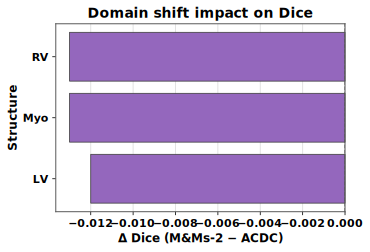
\includegraphics[width=0.72\linewidth]{figs/domain_shift.png}
\caption{Domain shift analysis: $\Delta$Dice per structure (M\&Ms‑2 minus ACDC).}
\label{fig:domain}
\end{figure}

\subsection{Diagnosis with KI‑GCN and calibration}
Using SKIF‑Seg masks, KI‑GCN attains 94.0\% accuracy and macro‑F1 0.93 across five ACDC classes. 
Macro ROC‑AUC and PR‑AUC are $\approx 0.964$ and $\approx 0.951$, respectively (Figure~\ref{fig:rocpr}). 
The normalized confusion matrix (Figure~\ref{fig:cm}) reveals balanced performance across classes. 
Post‑hoc temperature scaling ($\tau{=}2.1$) reduces over‑confidence, improving Brier from 0.08 to 0.07 and ECE from 0.04 to 0.03 (Figure~\ref{fig:reliability}), aligning with best practices in clinical AI~\cite{niculescu2005calibration,brier1950}.

\begin{figure}[!ht]
\centering
\includegraphics[width=0.48\linewidth]{figs/roc_curve.png}\hfill
\includegraphics[width=0.48\linewidth]{figs/pr_curve.png}
\caption{Macro ROC and PR curves for KI‑GCN on ACDC.}
\label{fig:rocpr}
\end{figure}

\begin{figure}[!ht]
\centering
\includegraphics[width=0.72\linewidth]{figs/confusion_matrix.png}
\caption{Normalized confusion matrix across five diagnostic classes.}
\label{fig:cm}
\end{figure}

\begin{figure}[!ht]
\centering
\includegraphics[width=0.72\linewidth]{figs/reliability_pre_post.png}
\caption{Reliability diagram before and after temperature scaling.}
\label{fig:reliability}
\end{figure}

\subsection{Throughput and portability}
Figure~\ref{fig:ep} summarizes inference throughput by EP. 
CUDA and DirectML provide $4$–$7\times$ acceleration over CPU with similar memory footprints and high pass‑rates for model graphs, enabling responsive inference on commodity hardware and broad deployment in mixed environments~\cite{onnxruntime_docs,cuda_guide,directml_docs}.

\begin{figure}[!ht]
\centering
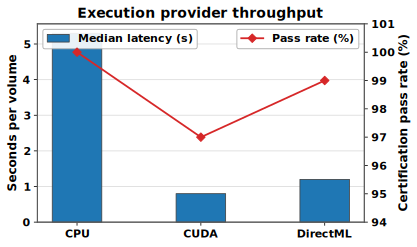
\includegraphics[width=0.72\linewidth]{figs/ep_throughput.png}
\caption{Inference throughput by execution provider (lower is better).}
\label{fig:ep}
\end{figure}



\section{Discussion}
\subsection*{Comparison with prior studies}
Our results align with prior segmentation literature: nnU‑Net consistently sets the state of the art on ACDC with a mean Dice of about 0.94, and MedNeXt reaches similar values using modernized ConvNet blocks~\cite{isensee2021nnunet,roy2023mednext}. 
SKIF‑Seg approaches these numbers while maintaining an emphasis on standards compliance, cross‑hardware execution, and manifest logging—capabilities often omitted from research code but essential for clinical use. 
On diagnosis, GNN‑based reasoning over segmentation‑derived features delivers high accuracy with interpretable pathways: edges correspond to anatomical or physiological couplings (e.g., LV\_ED↔LV\_ES), and node features are familiar clinical indices. 
This stands in contrast to direct image‑based classification models whose intermediate representations are difficult to map to clinical concepts.

\subsection*{Advantages and disadvantages}
\textbf{Advantages.} The system integrates privacy‑preserving ingestion, portable ONNX inference, and graph‑structured diagnosis in a single pipeline. 
It produces calibrated probabilities and a complete audit trail via manifests, increasing trust and reproducibility. 
Selective knowledge infusion—through anatomy‑aware post‑processing and graph edges—yields interpretable improvements without heavy model complexity. 
\textbf{Disadvantages.} The graph topology is predominantly expert‑defined, which stabilizes learning when labels are scarce but may restrict the discovery of novel biomarkers or interactions. 
Because diagnosis depends on segmentation, errors in thin‑wall myocardium or RV trabeculation can perturb derived features and degrade classification. 
While temperature scaling improves overall calibration, subgroup‑specific miscalibration may persist and requires targeted remedies.

\subsection*{Limitations, challenges, and open questions}
Three challenges remain. 
(1) \emph{Adaptive graph structure.} Learning edges jointly with node embeddings—subject to physiologic priors—could reveal latent relationships while preserving interpretability. 
(2) \emph{Robust generalization.} Small average performance drops can mask hidden stratification across vendors, protocols, or comorbidities; stratified evaluation and domain adaptation should be explored systematically on M\&Ms‑2~\cite{campello2021mnms,martinisla2023mnms2}. 
(3) \emph{Trust and calibration.} Temperature scaling is global; proximity‑informed or subgroup‑aware calibration may yield more equitable reliability across populations~\cite{xiong2023procal}. 
Finally, a prospective multi‑site study is needed to confirm clinical utility under routine conditions.



\section{Conclusion}
We presented a knowledge‑integrated system for cardiac MRI that combines standards‑compliant DICOM/NIfTI ingestion with de‑identification, ONNX‑portable volumetric segmentation (SKIF‑Seg), and graph‑based diagnostic reasoning (KI‑GCN). 
The pipeline is engineered for clinical reality: it respects interoperability standards, runs efficiently across CPUs and GPUs via ONNX Runtime execution providers, records a manifest with all key parameters and metrics for auditability, and produces calibrated probabilities to support decision‑making. 
On two public benchmarks, the system delivers competitive accuracy and robust generalization. 
On ACDC, SKIF‑Seg improves a strong U‑Net baseline and achieves macro Dice 0.939 with per‑structure Dice of 0.965 (LV), 0.912 (Myo), and 0.941 (RV) and lower boundary error (HD95 reduced by ≈1.7 mm). 
On M\&Ms‑2, it maintains high accuracy with small, uniform Dice drops, indicating resilience to cross‑center domain shift. 
The downstream KI‑GCN classifier achieves 94.0\% accuracy with macro ROC‑AUC ≈0.964 and macro PR‑AUC ≈0.951; post‑hoc temperature scaling reduces the Brier score from 0.08 to 0.07 and ECE from 0.04 to 0.03, improving reliability without sacrificing discrimination. 
Throughput results show that CUDA and DirectML offer $4$–$7\times$ faster inference than CPU while retaining broad hardware coverage, enabling deployment on commodity clinical workstations and research laptops alike.

Two limitations define an agenda for future work. 
First, the graph topology in KI‑GCN is expert‑specified. 
Integrating data‑driven edge learning with physiologic priors could expose subtle relationships between structures and phases, improving diagnostic sensitivity while preserving interpretability. 
Second, the two‑stage design propagates segmentation errors into diagnosis; explicit uncertainty quantification, active learning, and human‑in‑the‑loop correction are natural remedies. 
Additional directions include stronger domain adaptation across vendors and sequences, proximity‑informed or subgroup‑aware calibration to improve fairness, and a prospective multi‑site study evaluating end‑to‑end workflow impact (time‑to‑report, inter‑reader agreement, and user trust). 
By treating \emph{knowledge} as a first‑class engineering primitive—embedded in standards, algorithms, and evaluation—the proposed system offers a practical blueprint for turning high‑performing research code into portable, auditable, and trustworthy clinical software.


\bibliography{references}

\end{document}
